\documentclass{article}
\usepackage{tikz}
\usepackage{adjustbox}

\begin{document}

{\ttfamily \textbf{UNITED STATES}} \\
{\ttfamily \textbf{AIR STATUS DISPLAY}}

\vspace{1em}

{\ttfamily \textbf{Date of}} \\
{\ttfamily \textbf{Mission}}

\begin{adjustbox}{center}
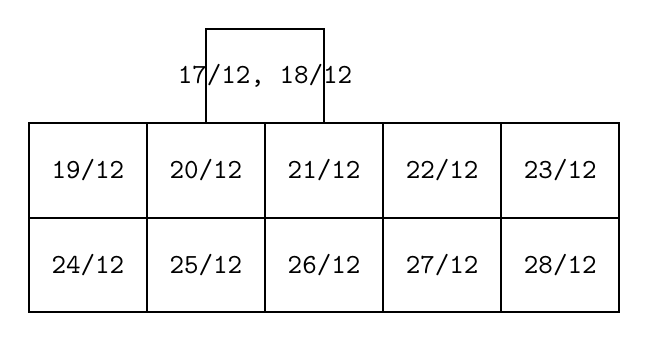
\begin{tikzpicture}
    % Define box size
    \def\boxwidth{1.5}
    \def\boxheight{1.2}

    % Define mission dates with correct layout
    \def\dates{
        {24/12, 25/12, 26/12, 27/12, 28/12},
        {19/12, 20/12, 21/12, 22/12, 23/12},
        {17/12, 18/12}
    }

    % Draw the grid with offset for the bottom row
    \foreach \row [count=\y from 0] in \dates {
        \foreach \date [count=\x] in \row {
            \pgfmathsetmacro\xpos{\x - 1}  % Adjust horizontal position
            \pgfmathsetmacro\ypos{2 - \y}  % Adjust vertical position
            
            % Offset bottom row (first row in data)
            \ifnum\y=2
                \pgfmathsetmacro\xpos{\xpos + 1.5}  % Shift right for alignment
            \fi

            \draw[thick] (\xpos*\boxwidth, -\ypos*\boxheight) 
                rectangle (\xpos*\boxwidth + \boxwidth, -\ypos*\boxheight - \boxheight);
            \node at (\xpos*\boxwidth + 0.75, -\ypos*\boxheight - 0.6) {\ttfamily \textbf{\date}};
        }
    }
\end{tikzpicture}
\end{adjustbox}

\end{document}
